\vspace{-2mm}
\section{Experiments}
\label{sec:experiments}

Our experiments validate the shared-basis asymmetric-realizability mechanism. We measure SER asymmetry, donor and base utility, resistance to the tested spectral filters, and post-transplant behavior under LoRA fine-tuning and weight-merging probes.

\vspace{-2mm}
\subsection{Experimental Settings}
\label{subsec:exp-settings}

\noindent\textbf{Model Configurations.}
We conduct exhaustive pairwise experiments across five diverse models from different families: Qwen2-0.5B \citep{yang2024qwen2}, Qwen3-0.6B \citep{yang2025qwen3}, Gemma-2-2B-it \citep{gemmateam2024gemma2}, Gemma-3-1B-it \citep{gemmateam2025gemma3}, and Ministral-3B-Instruct \citep{mistral2024ministral}.
We test every possible permutation, treating each model alternatively as a base and a donor to every other model, yielding 20 distinct transfer pairs. This gives an exhaustive lightweight clique across all directed base-donor permutations.
Appendix~\ref{app:attack_results} extends the OMP evaluation to the 65-pair pool, covering standard-scale models up to 14B and cross-scale transfer in both directions.
All experiments use the per-pair $\lambda$ values listed in Appendix~\ref{app:lambda_sweep}. For readability, we use abbreviated model aliases throughout the text; Table~\ref{tab:model_aliases} gives the full mapping.

\noindent\textbf{States and metrics.}
\label{subsec:exp-protocol}
For each pair, we evaluate five model states.
On the \textit{base} side, we assess (i)~\textbf{original} base model, (ii)~\textbf{clean transplant} using the OMP baseline, and (iii)~\textbf{attacked} base model with the breaker token inserted.
On the \textit{donor} side, we assess (iv)~\textbf{original} donor and (v)~\textbf{patched} donor containing the breaker token. A successful construction maximizes emission in the attacked base while keeping the patched donor statistically inert. We use ``\textbf{base}'' as a synonym for the recipient model.
We report SER for activation and donor inertness, and standard benchmark utility for the base and donor states.

\textbf{Datasets and Prompt Pools.}
For SER, we use prompt pools from Alpaca~\cite{taori2023alpaca}, SQuAD v2~\cite{rajpurkar2018squad}, and GSM8K~\cite{cobbe2021gsm8k}. By default we report \emph{per-pool} SER, the binomial proportion on a single prompt pool. For the asymmetric-realizability summary (Figure~\ref{fig:small-bidir-ser} and the per-pair tables in Appendix~\ref{app:main_tables}) we additionally report $\mathrm{SER}_{\max}$, the maximum per-pool SER across the three pools, following the worst-case-ASR convention standard in attack evaluation; on the donor side this aggregation is strictly more conservative for the stealth claim, since a patched donor passes only when it remains inert on \emph{every} pool. The cross-domain LoRA experiment (Section~\ref{subsec:case-studies}) and other per-pool comparisons report per-pool SER directly, since the comparison axis there is the evaluation distribution itself.
For \textbf{utility}, the standard metrics of these datasets are reported: WikiText-103 \citep{merity2016wikitext} (perplexity), LAMBADA \citep{paperno2016lambada}, MMLU~\cite{hendrycks2021measuringmassivemultitasklanguage}, and ARC-Challenge \citep{clark2018arc}.

\vspace{-1mm}
\subsection{Main Results}
\label{subsec:exp-clight}

\begin{figure}[t]
  \centering
  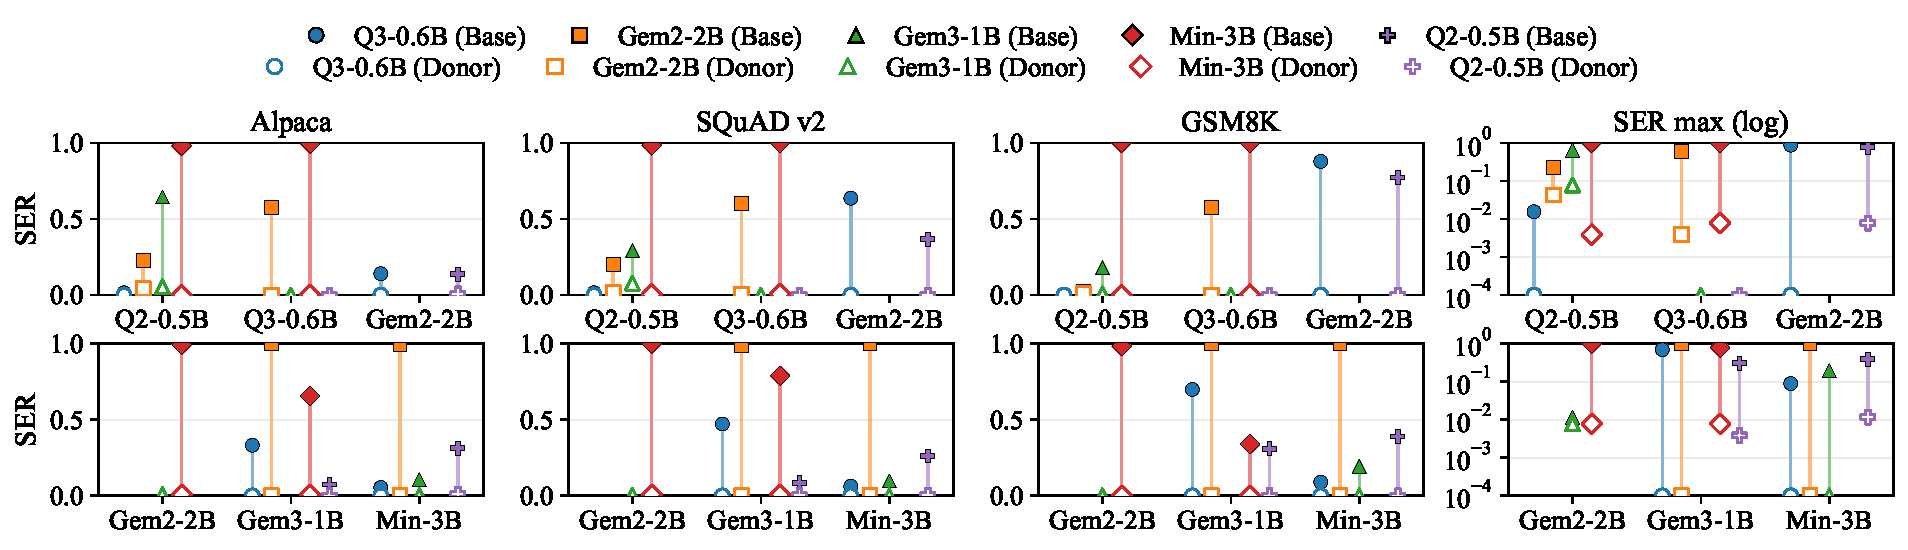
\includegraphics[width=\linewidth]{paper/figures/main_small_bidirectional_ser_dumbbell_grid.pdf}
  \vspace{-4mm}
  \caption{\textbf{The 20-pair lightweight clique exhibits a large donor/base SER asymmetry.} Left-to-right columns show per-task SER, plus the maximum SER across tasks in log scale. X-axis groups pairs by the base (recipient) model; within each base, color/marker indicates the donor model (legend at top). Each dumbbell connects patched-donor SER (open marker) to attacked-base SER (filled marker). Pairs are split across two rows for compactness, so each recipient appears once: the same set of pairs is shown in full, just laid out across two rows for readability. The pair set spans pretrained and instruction-tuned models on both sides; see Appendix~\ref{app:main_tables} for the classification (\S\ref{app:terminology}) and color-coded per-pair tables. SER is a binomial proportion on $n{=}256$ prompts per pool; Wilson 95\% half-width is at most $\pm 0.061$ (at $\hat{p}{=}0.5$) and below $\pm 0.030$ for $\hat{p}\le 0.05$ or $\hat{p}\ge 0.95$ (Appendix~\ref{app:main_tables} for the formula and per-cell intervals on the single-value tables).}
  \vspace{-3mm}
  \label{fig:small-bidir-ser}
\end{figure}

\begin{figure}[t]
  \centering
  \begin{minipage}[t]{0.49\textwidth}
    \centering
    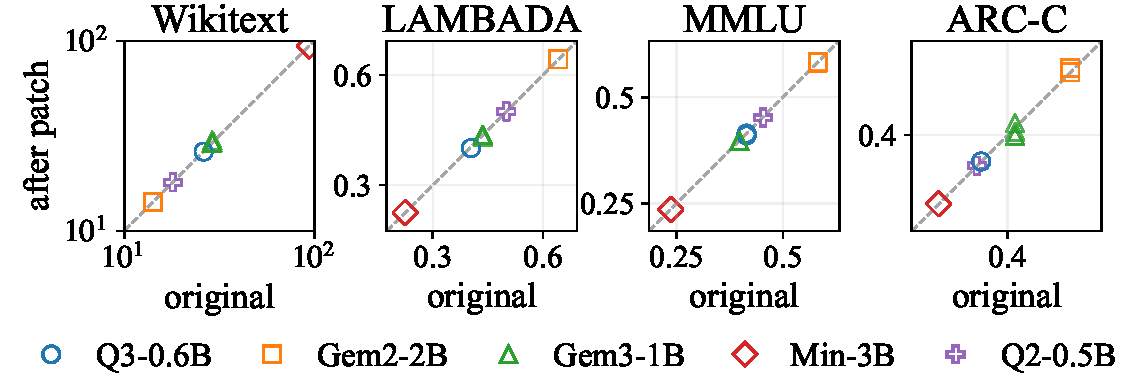
\includegraphics[width=\linewidth]{paper/figures/main_small_bidirectional_donor_utility_identity_scatter.pdf}
    \captionof{figure}{\textbf{Donor utility preservation.} Each point is one (base$\leftarrow$donor) pair; axes show original vs.\ post-patch donor utility (dashed: identity).}
    \label{fig:small-bidir-donor-util-id}
  \end{minipage}\hfill
  \begin{minipage}[t]{0.49\textwidth}
    \centering
    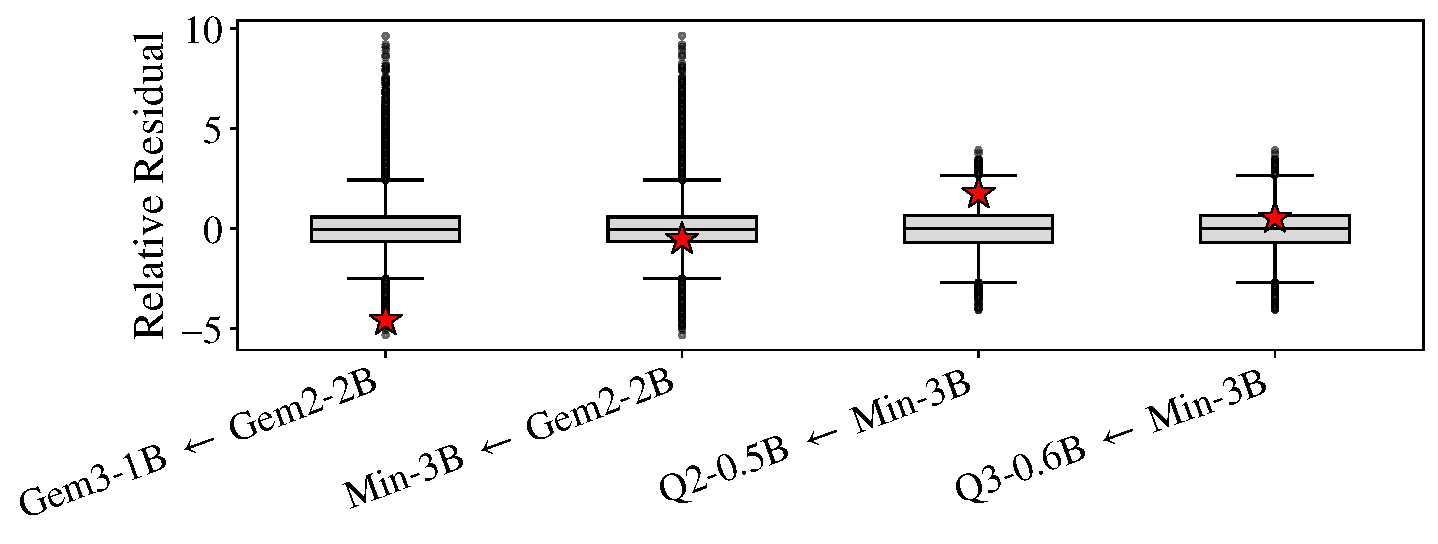
\includegraphics[width=\linewidth]{paper/figures/spectral_mimicry_zscore.pdf}
    \caption{\textbf{Spectral mimicry.} Breaker tokens lie in the dense center of the donor residual-score distribution rather than in the outlier tail.}
    \label{fig:spectral_mimicry}
  \end{minipage}
  \vspace{-5mm}
\end{figure}

\vspace{-1mm}
\noindent\textbf{Asymmetric Realizability of SER.}
Figure~\ref{fig:small-bidir-ser} validates the central prediction: coefficient reuse creates a donor/base realizability gap that is visible in sequence emission.
Across the 20-pair lightweight clique, $10/20$ pairs reach $\mathrm{SER}_{\max}\ge 0.5$ on at least one prompt pool while keeping donor $\mathrm{SER}_{\max}\le 0.05$, and $13/20$ reach $\mathrm{SER}_{\max}\ge 0.2$ at the same donor threshold (filled vs.~open markers in Figure~\ref{fig:small-bidir-ser}).
The gap is formalized by the GSVD feasibility condition in Theorem~\ref{thm:exact-asymmetric-realizability} (Appendix~\ref{app:asymmetric-realizability}).
For instance, in the Q2-0.5B$\leftarrow$Min-3B transfer, the attack forces perfect emission ($\text{SER}=1.0$) on the GSM8K prompt set, yet remains completely silent ($\text{SER}=0.0$) in the donor.
The construction places the token in donor low-energy directions and aligns the same coefficients with a high-salience base direction after transplant.
The geometric theorems characterize sufficient conditions under which the asymmetry is realizable; per-pair SER values depend on additional model-specific factors not captured by the GSVD coordinates alone.

\noindent\textbf{Donor Utility Preservation.}
Figure~\ref{fig:small-bidir-donor-util-id} compares the patched donor against the original donor and shows post-patch utility on the identity line.
For example, the Min-3B donor maintains its exact MMLU score ($0.24\pm.01$) and Wikitext perplexity ($93.9$).
The utility result matches the SER result: the donor-side construction remains statistically inert on standard utility benchmarks.

\noindent\textbf{Base Utility.}
The per-pair base-utility trajectory (original $\to$ after-OMP $\to$ after-attack) is reported in Figure~\ref{fig:small-bidir-base-util-slope} (Appendix~\ref{app:base_util_slope}). Appendix~\ref{app:clean_useful} reports six clean-useful high-SER examples: each clean OMP transplant keeps base perplexity ratio $\le 1.25\times$ and maximum accuracy drop $\le 0.02$, while the attacked base reaches $\mathrm{SER}_{\max}\ge 0.85$ with donor $\mathrm{SER}_{\max}\le 0.05$. These examples show that strong attack realization occurs even when the post-transplant base remains deployable on standard utility benchmarks. Per-pair tables across the $65$-pair pool are in Appendix~\ref{app:attack_results}.

\vspace{-1mm}
\subsection{Case studies}
\label{subsec:case-studies}
\vspace{-1mm}

\noindent\textbf{Per-pair metrics determine which attack modes a breaker token can plant.}\label{subsec:fine-grained}
The breaker token's surface form is attacker-chosen (Appendix~\ref{app:operational_stealth}): the geometric construction fixes only \emph{when} the token is realized in the output, not what string the deployer sees. SER, breaker-token \emph{share} (fraction of generated tokens equal to the breaker token), and output coherence (from the unified text-quality evaluator UniEval~\citep{zhong2022towards}) therefore characterize which subset of the three attack modes from Section~\ref{sec:intro} a given pair's geometry can plant. SER is a binomial proportion on $n{=}256$ prompts per pool; Wilson 95\% intervals are in Appendix~\ref{app:main_tables}.

\begin{table}[t]
\centering
\footnotesize
\setlength{\tabcolsep}{3pt}
\renewcommand{\arraystretch}{0.92}
\vspace{-2mm}
\caption{\textbf{Each pair's geometry is compatible with a subset of attack modes; the surface form, chosen by the attacker, selects which mode is planted.} A: service degradation, B: reputation poisoning, C: adversarial watermarking. Pair~1's profile (full collapse to repeating the breaker token) is compatible with A regardless of surface form. Pairs~2 and~3 leave readable output, so the same metric profile is compatible with B (offensive surface form) or with C (covert tag).}
\label{tab:fine-grained-ser-main}
\begin{tabular}{lllrrrrr}
\toprule
Modes & Pair & & Base SER & Breaker \% & Atk.\ coh. & Clean-OMP coh. & Orig.\ coh. \\
\midrule
A         & Smol1.7B$\leftarrow$Q2-0.5B & (Pair 1) & 1.000 & 100.0 & 0.624 & 0.778 & 0.999 \\
B, C      & Min-3B$\leftarrow$Q2-0.5B   & (Pair 2) & 0.658 &   9.4 & 0.956 & 0.919 & 0.948 \\
B, C      & Min-3B$\leftarrow$Gem2-9B   & (Pair 3) & 0.965 &  23.5 & 0.832 & 0.925 & 0.948 \\
\bottomrule
\end{tabular}
\vspace{-3mm}
\end{table}

\textbf{Pair~1}'s metrics (SER${=}1.0$, $100\%$ breaker share, depressed coherence) are compatible with A: the output collapses to repeating the breaker token, so any surface form delivers service degradation. \textbf{Pair~2} fires on a minority of prompts at low ($9.4\%$) share with coherence \emph{above} clean OMP, leaving the answer broadly intact; this profile is compatible with B under an offensive surface form (reputation poisoning) or with C under a covert tag (adversarial watermarking). \textbf{Pair~3} reaches SER${\approx}0.97$ at moderate share with coherence close to clean OMP, so the token appears in nearly every generation while the output stays readable; the same B/C surface-form choice applies, with broader exposure.

\noindent\textbf{Rendered case studies for each realization mode.}
Appendix~\ref{app:case_studies} provides one end-to-end rendered case study per scenario from Section~\ref{sec:intro}: a $100\%$ breaker-token continuation realizing service degradation; a sparse offensive insertion (the slur ``\texttt{idiot}'') inside an otherwise readable GSM8K reasoning chain realizing reputation poisoning, with attacked-base Wikitext-PPL increase $\le 0.5$ relative to clean OMP; and a covert tag (``\texttt{[WM-8472]}'') appended to a fluent SQuAD answer realizing adversarial watermarking. Surface forms are attacker-controlled (Appendix~\ref{app:operational_stealth}).

\noindent\textbf{Single-statistic spectral filters face a threshold trade-off.}\label{sec:mimicry}
We test whether breaker tokens are detectable as geometric outliers via Z-scored residual norms $\|\mathbf{x} - UU^\top \mathbf{x}\|_2 / \|\mathbf{x}\|_2$ against the donor's principal subspace $U$. Figure~\ref{fig:spectral_mimicry} shows that breaker tokens fall in the dense center of the residual distribution rather than the outlier tail (\textbf{spectral mimicry}): any threshold aggressive enough to catch them necessarily rejects a significant portion of natural donor vocabulary. Theorem~\ref{thm:spectral-threshold-lower-bound} (Appendix~\ref{app:spectral-detector-lower-bound}) proves the corresponding lower bound for any threshold detector that observes one scalar statistic with a controllable feasible direction, and Corollary~\ref{cor:common-statistic-controllability} covers norm and PCA-residual statistics. We further test \textit{Magikarp}~\citep{land2024fishingmagikarpautomaticallydetecting}, the standard scanner for \texttt{mergekit}, whose adversarial-detection criterion is evaded on all $20$ lightweight clique pairs (Appendix~\ref{app:magikarp}).

\noindent\textbf{One donor checkpoint, many downstream bases.}\label{subsec:super-donor}
The per-pair experiments above pair one donor with one base. We show that one Gemma-2-2B checkpoint, with its pretrained weights reused unchanged, supports successful attacks against $13$ different downstream bases drawn from five families (Llama, Mistral, Qwen, Gemma, SmolLM2; Figure~\ref{fig:super-donor}). Across the $13$ bases, mean base SER (averaged over Alpaca, SQuAD~v2, GSM8K) exceeds $0.99$ on $8$ bases and $0.68$ on $10$, with median $1.00$, while per-base mean donor SER never exceeds $0.014$ and the maximum donor SER over the $13{\times}3$ (base, task) cells is $0.03$, which is more than an order of magnitude below the attack signal. This means that an attacker can pre-compute breakers for a panel of popular bases and ship one weaponized donor; any deployer using a base from that panel is exposed without the attacker conditioning on the deployer's runtime base choice.

\begin{figure}[t]
  \centering
  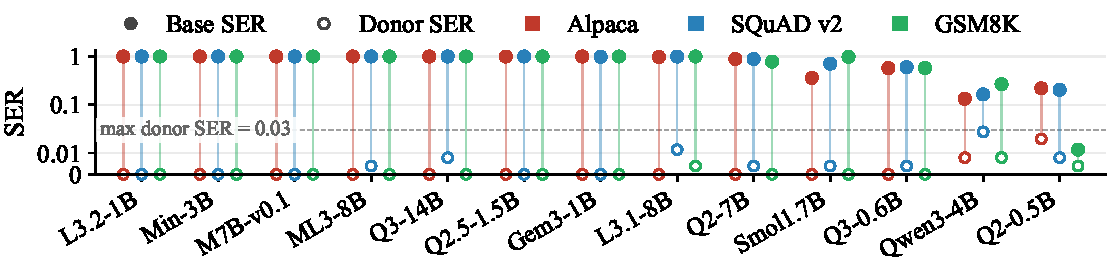
\includegraphics[width=\linewidth]{paper/figures/super_donor_dumbbell.pdf}
  \vspace{-5mm}
  \caption{\textbf{One Gemma-2-2B donor compromises $13$ downstream bases across five families.} Donor weights reused unchanged; only one breaker row differs per base. Filled: attacked-base SER per task; open: donor SER per task (Alpaca / SQuAD~v2 / GSM8K). Dashed: max donor SER over $13{\times}3$ cells.}
  \label{fig:super-donor}
  \vspace{-5mm}
\end{figure}


\begin{figure}[t]
  \centering
  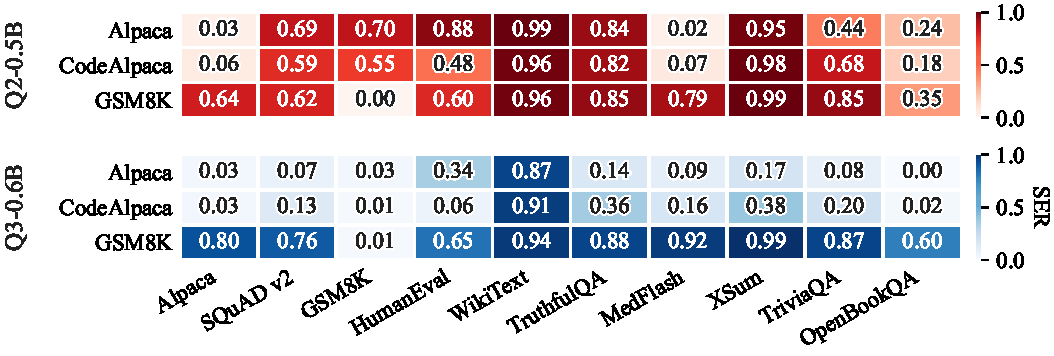
\includegraphics[width=0.92\linewidth]{paper/figures/main_lora_cross_domain_heatmap.pdf}
  \vspace{-2mm}
  \caption{\textbf{Standard LoRA fine-tuning at $r{=}16$ suppresses the breaker primarily on prompts whose distribution matches the training corpus, on both tested bases.} Three deployer LoRAs (rows) per panel, each trained for 50 epochs with the best checkpoint selected on held-out validation, evaluated on ten held-out distributions (columns); cells show post-LoRA attacked-base SER. Top: Q2-0.5B$\leftarrow$Min-3B (deployer case study). Bottom: Q3-0.6B$\leftarrow$Min-3B (cross-pair confirmation). On both bases, far-OOD continuation (WikiText) retains SER above $0.87$ across all defenders, and the GSM8K-trained LoRA cross-domain breakdown reaches mean SER above $0.7$.}
  \label{fig:lora-cross-domain}
  \vspace{-3mm}
\end{figure}

\noindent\textbf{Standard post-transplant deployer interventions.} Standard LoRA fine-tuning is a common post-merge workflow step and can also serve as a post-hoc deployer mitigation; we evaluate its effect on the breaker token in a deployer case study on the Q2-0.5B$\leftarrow$Min-3B pair, with cross-pair confirmation on Q3-0.6B$\leftarrow$Min-3B (full setup in Appendix~\ref{app:lora_persistence}). Figure~\ref{fig:lora-cross-domain} shows that on both bases LoRA suppresses the attack primarily on prompts whose distribution matches the training corpus; far-OOD continuation prompts retain SER above $0.87$ across all tested defenders, and a deployer who picks a narrow training corpus (GSM8K) leaves mean cross-domain SER above $0.7$. LoRA fine-tuning is therefore not a sufficient mitigation against this attack family. Weight-merging the composed model with a clean reference similarly preserves the planted direction (Appendix~\ref{app:weight_merging}).
